\chapter{Implementation}
\label{chap:implementation}
	\textit{This chapter shows the implementation and deployment processes, including system frameworks and system specifications.}
\minitoc

\section{Tiền xử lý dữ liệu} 
\label{sec:tien_xu_ly_du_lieu}
	Trong mục này, chúng tôi trình bày các công việc chúng tôi sẽ thực hiện trên tập dữ liệu trước lúc sử dụng cho quá trình huấn luyện bao gồm nội suy dữ liệu, trích xuất thành phần gan và biến đổi cường độ sáng điểm ảnh.

\subsection{Nội suy dữ liệu} 
\label{subsec:noi_suy_du_lieu}
	Khi xem xét thông số kích thước điểm ảnh trong khối ảnh CT (cột thứ ba \autoref{tab:3d_ircadb_01_info}), chúng tôi nhận thấy kích thước điểm ảnh giữa các bộ ảnh CT là khác nhau, đặc biệt khoảng cách giữa hai lớp ảnh CT ở một số bộ ảnh rất lớn. Điều này không tốt cho việc học của lớp convolution\index{Convolution} bởi tính chất khai thác thông tin về cấu trúc không gian của nó. Chúng tôi thực hiện nội suy dữ liệu như mô phỏng ở \autoref{fig:interpolation}. Ở đây chúng tôi sử dụng nội suy bậc ba với hàm \verb/zoom/ trong gói \verb/ndimage/ của thư viện \verb/scipy/ trong Python với kích thước đầu ra của mỗi điểm ảnh là 1mm(W)$\times$1mm(H)$\times$1mm(D).
	\begin{figure}[h!]
		\centering
		\begin{tikzpicture}[scale=.4]
	% \drawtile#x#y#size#drawcolor
	\def\drawtile#1#2#3#4{
		\filldraw[fill=black, fill opacity=.3, draw=#4] (#1, #2) -- (#1 + #3, #2) -- (#1 + 1.5 * #3, #2 + #3 / 2) -- (#1 + #3 / 2, #2 + #3 / 2) -- cycle;
	}
	
	% \drawline#x1#y1#x2#y2#color
	\def\drawline#1#2#3#4#5{
		\draw[#5] (#1, #2) -- (#3, #4);
	}
	
	% interpolation
	\foreach \x in {0, 20} {
		\foreach \y in {0, ..., 4} {
			\drawtile{\x}{\y}{7}{black}
			\ifnum\x=20
				\ifnum\y<4
					\drawtile{\x}{\y + .5}{7}{none}
					\drawline{30.75}{4 + \y}{32}{5.5}{gray}
				\fi
			\fi
		}
	}
	\draw[->, ultra thick] (12, 3.75) -- (18, 3.75) node[midway, above] {Nội suy};
	\node at (36, 5.5) {Các lớp nội suy};
\end{tikzpicture}
		\caption[Nội suy được sử dụng để lấp các lớp bị thiếu trong khối ảnh CT.]{Nội suy được sử dụng để lấp các lớp bị thiếu trong khối ảnh CT (Nguồn \cite{sach2017interpolation}).}
		\label{fig:interpolation}
	\end{figure}

\subsection{Trích xuất thành phần gan} 
\label{subsec:trich_xuat_thanh_phan_gan}
	Từ kết quả khảo sát tình trạng bộ dữ liệu (\autoref{tab:3d_ircadb_01_state}), chúng tôi nhận thấy việc sử dụng khối ảnh CT gốc cho việc huấn luyện là bất khả thi vì nhãn phân đoạn cho động mạch ở một số bệnh nhân không được cung cấp. Tuy nhiên, phần động mạch trong cơ quan gan là không đáng kể và hầu hết động mạch đều nằm bên ngoài gan, chúng tôi đề xuất thực hiện trích xuất thành phần gan và chỉ sử dụng thành phần này để huấn luyện hệ thống. \autoref{fig:pre_processing_extract} mô tả việc trích xuất thành phần gan trong khối ảnh CT nhờ sử dụng nhãn phân đoạn gan được cung cấp. 
	\begin{figure}[h!]
		\begin{subfigure}[b]{0.24\textwidth}
			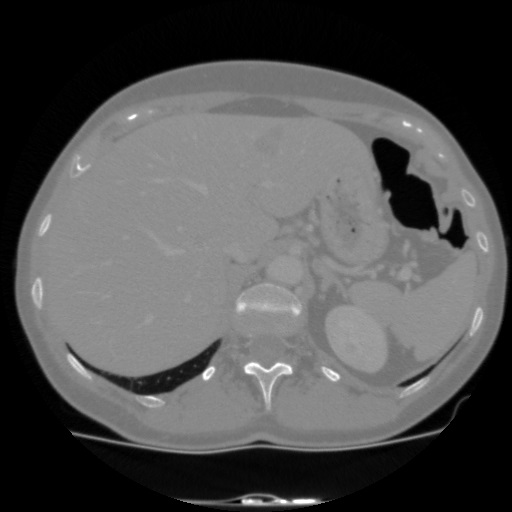
\includegraphics[width=\textwidth]{figures/pre_processing_extract_dicom}
			\caption{}
			\label{fig:pre_processing_extract_dicom}
		\end{subfigure}
		\hfill
		\begin{subfigure}[b]{0.24\textwidth}
			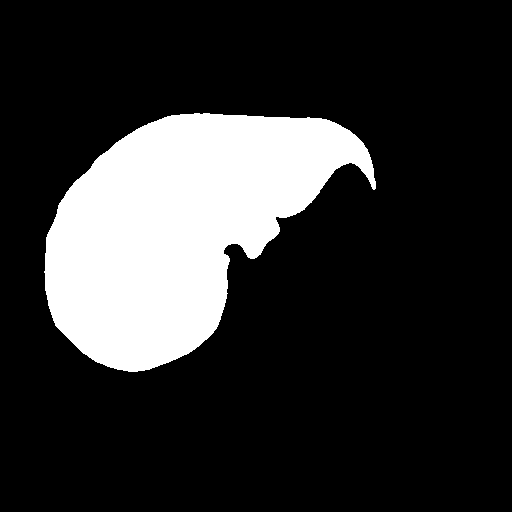
\includegraphics[width=\textwidth]{figures/pre_processing_extract_liver}
			\caption{}
			\label{fig:pre_processing_extract_liver}
		\end{subfigure}
		\hfill
		\begin{subfigure}[b]{0.24\textwidth}
			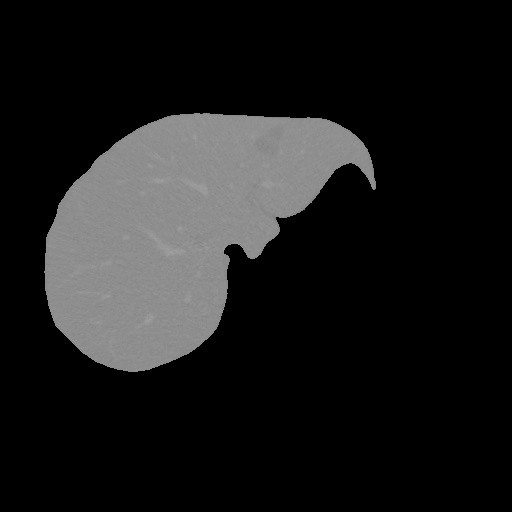
\includegraphics[width=\textwidth]{figures/pre_processing_extract_crop}
			\caption{}
			\label{fig:pre_processing_extract_crop}
		\end{subfigure}
		\hfill
		\begin{subfigure}[b]{0.24\textwidth}
			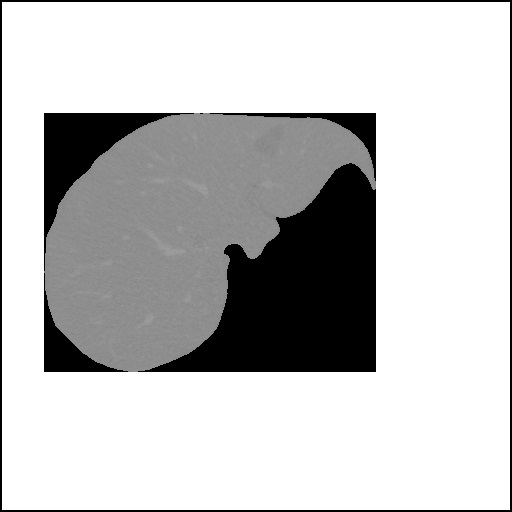
\includegraphics[width=\textwidth]{figures/pre_processing_extract_done}
			\caption{}
			\label{fig:pre_processing_extract_done}
		\end{subfigure}
		\caption[Mô phỏng quá trình trích xuất thành phần gan trong khối ảnh CT.]{Mô phỏng quá trình trích xuất thành phần gan trong khối ảnh CT. \subref{fig:pre_processing_extract_dicom} ảnh CT gốc. \subref{fig:pre_processing_extract_liver} nhãn phân đoạn gan được sử dụng để trích xuất thành phần gan trong ảnh CT. \subref{fig:pre_processing_extract_crop} phần ảnh CT chứa gan sau trích xuất. \subref{fig:pre_processing_extract_done} thu giảm kích thước dữ liệu bằng cách giữ lại khối dữ liệu nhỏ nhất chứa gan.}
		\label{fig:pre_processing_extract}
	\end{figure}

	Từ đây trở đi, hệ thống của chúng tôi sẽ đặt trên một giả thiết rằng nhãn phân đoạn cơ quan gan đã biết trước và hệ thống chỉ phân đoạn hệ thống mạch máu bên trong cơ~quan~gan.

\newpage
\subsection{Biến đổi cường độ sáng} 
\label{subsec:bien_doi_cuong_do_sang}
	Chúng tôi thực hiện biến đổi cường độ sáng điểm ảnh với mong muốn làm rõ hình ảnh mạch máu trên dữ liệu đầu vào, giúp quá trình học dễ dàng hơn. Chúng tôi tiến hành phân tích phân phối mức sáng của các điểm ảnh trong cơ quan gan. \autoref{fig:pre_processing_histogram} là biểu đồ phân phối mức sáng nền gan và mạch máu gan của hai đại diện là bệnh nhân số 5 và bệnh nhân số 8.
	\begin{figure}[h!]
		\centering
		\begin{subfigure}[b]{.8\textwidth}
			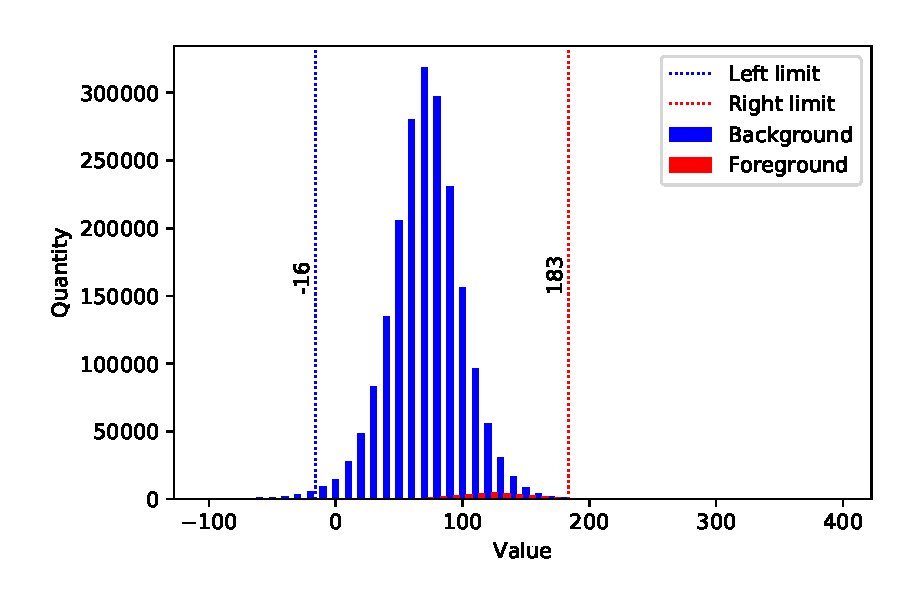
\includegraphics[width=\textwidth]{figures/pre_processing_histogram_5}
			\caption{}
			\label{fig:pre_processing_histogram_5}
		\end{subfigure}\\[5mm]
		\begin{subfigure}[b]{.8\textwidth}
			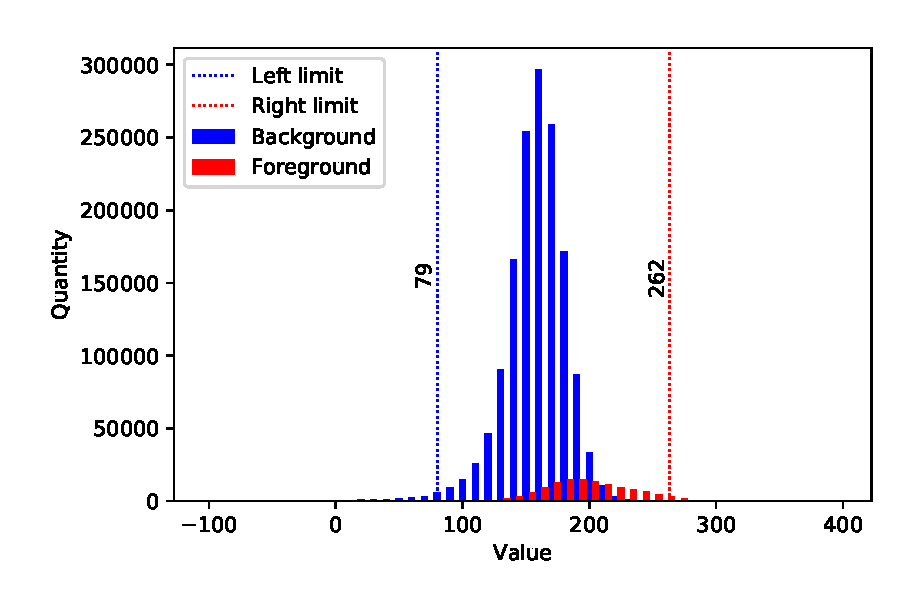
\includegraphics[width=\textwidth]{figures/pre_processing_histogram_8}
			\caption{}
			\label{fig:pre_processing_histogram_8}
		\end{subfigure}
		\caption[Phân phối mức sáng của các điểm ảnh thuộc nền cơ quan gan và mạch máu gan cùng ngưỡng giới hạn trái và phải.]{Phân phối mức sáng của các điểm ảnh thuộc nền cơ quan gan (Background\index{Background}) và mạch máu gan (Foreground\index{Foreground}) cùng ngưỡng giới hạn trái (Left limit\index{Left limit}) và phải (Right limit\index{Right limit}). \subref{fig:pre_processing_histogram_5} bệnh nhân số 5. \subref{fig:pre_processing_histogram_8} bệnh nhân số 8.}
		\label{fig:pre_processing_histogram}
	\end{figure}	
	Từ biểu đồ chúng ta thấy phân phối mức sáng trên các bệnh nhân khác nhau có sự chênh lệch. Tuy nhiên, phân phối này có dạng phân phối chuẩn. Chúng tôi đề xuất thực hiện chuẩn hoá để đưa dữ liệu về cùng một phân phối. Chúng tôi thực hiện tính các giá trị ngưỡng bao gồm
	\begin{equation}
		Left\ limit = \mu - \alpha\sigma
		\label{eqn:left_threshold}
	\end{equation}
	và
	\begin{equation}
		Right\ limit = \mu + \beta\sigma.
		\label{eqn:right_threshold}
	\end{equation}
	Trong đó, $Left\ limit$\index{Left limit} là ngưỡng dưới, $Right\ limit$\index{Right limit} là ngưỡng trên, $\mu$ là giá trị trung bình và $\sigma$ là độ lệch chuẩn của các điểm ảnh trong khối cơ quan gan. Hai giá trị $\alpha$ và $\beta$ chúng tôi đề xuất lần lượt là 3 và 3.5. Giá trị $\beta$ cao hơn $\alpha$ do độ sáng của các điểm ảnh thuộc mạch máu hầu hết cao hơn độ sáng nền gan, mục đích giữ lại các điểm ảnh thuôc mạch máu có độ sáng cao. Chúng tôi áp dụng các giá trị ngưỡng trên dữ liệu đầu vào. Gọi $I^3$ là không gian khối dữ liệu, công thức áp dụng ngưỡng vào khối dữ liệu như sau
	\begin{equation}
		{P_1}_x=
		\begin{cases}
			Left\ limit, & \text{nếu}\ {P_0}_x < Left\ limit\\
			Right\ limit, & \text{nếu}\ {P_0}_x > Right\ limit\\
			{P_0}_x, & \text{còn lại},
		\end{cases}
		\label{eqn:apply_threshold}
	\end{equation} 
	trong đó, ${P_0}_x$ là giá trị điểm ảnh đầu vào và ${P_1}_x$ là giá trị điểm ảnh đầu ra tại toạ độ $x$ với $x\in I^3$. Sau đó, chúng tôi chuẩn hoá miền giá trị dữ liệu về khoảng 0 đến 1 theo công thức sau
	\begin{equation}
		{P_2}_x=\dfrac{{P_1}_x - Left\ limit}{Right\ limit - Left\ limit},
		\label{eqn:normalize_unit}
	\end{equation}
	trong đó, ${P_1}_x$ là giá trị đầu ra trong \autoref{eqn:apply_threshold} và ${P_2}_x$ là giá trị sau chuẩn hoá.

	Để hình ảnh mạch máu trở nên rõ hơn, chúng tôi tiến hành biến đổi giá trị mức sáng của các điểm ảnh theo công thức sau
	\begin{equation}
		{P_3}_x={P_2}_x^2.
		\label{eqn:normalize_gama}
	\end{equation}
	\autoref{fig:pre_processing_intensity} mô tả kết quả chuẩn hoá dữ liệu sau mỗi giai đoạn. So sánh kết quả trước và sau chuẩn hoá, chúng ta có thể thấy hình ảnh mạch máu đã trở nên rõ ràng hơn rất nhiều. Đây là cơ sở quan trọng giúp công tác huấn luyện đạt hiệu quả tốt hơn.
	\begin{figure}[h!]
		\begin{subfigure}[b]{0.32\textwidth}
			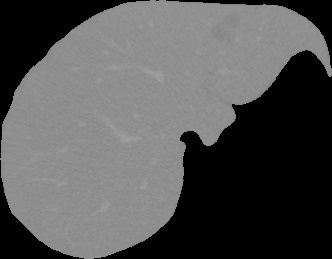
\includegraphics[width=\textwidth]{figures/pre_processing_intensity_origin}
			\caption{}
			\label{fig:pre_processing_intensity_origin}
		\end{subfigure}
		\hfill
		\begin{subfigure}[b]{0.32\textwidth}
			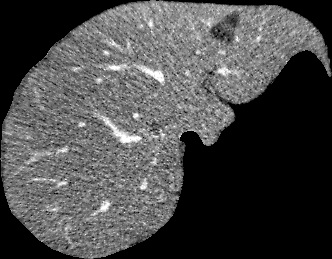
\includegraphics[width=\textwidth]{figures/pre_processing_intensity_clamp}
			\caption{}
			\label{fig:pre_processing_intensity_clamp}
		\end{subfigure}
		\hfill
		\begin{subfigure}[b]{0.32\textwidth}
			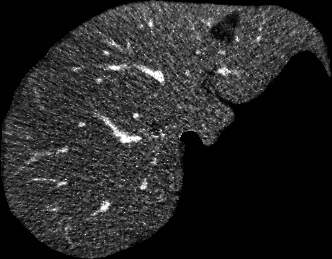
\includegraphics[width=\textwidth]{figures/pre_processing_intensity_gamma}
			\caption{}
			\label{fig:pre_processing_intensity_gamma}
		\end{subfigure}
		\caption[Biến đổi cường độ sáng điểm ảnh để làm rõ mạch máu.]{Biến đổi cường độ sáng điểm ảnh để làm rõ mạch máu. \subref{fig:pre_processing_intensity_origin} ảnh trước khi biến đổi. \subref{fig:pre_processing_intensity_clamp} ảnh sau khi thực hiện đặt ngưỡng trên và dưới. \subref{fig:pre_processing_intensity_gamma} biến đổi cường độ sáng bằng hàm bình phương giá trị điểm ảnh.}
		\label{fig:pre_processing_intensity}
	\end{figure}

\subsection{Làm giàu dữ liệu} 
\label{subsec:lam_giau_du_lieu}
	Khi huấn luyện một mạng học sâu, thực chất chúng ta đang học một hàm biến đổi có thể ánh xạ từ dữ liệu đầu vào tới nhãn tương ứng. Mô hình càng lớn, số lượng tham số cần học càng nhiều và quá trình huấn luyện đòi hỏi cần nhiều dữ liệu để đạt hiệu quả cao. Do đó, đối với những tập dữ liệu nhỏ, bước làm giàu dữ liệu có vai trò quan trọng trong việc cải thiện hiệu năng mô hình.
	
	Có nhiều cách làm giàu dữ liệu, ví dụ như phép lật hoặc xoay hình. Tuy nhiên, đối với ảnh y khoa như ảnh CT, những phép biến đổi này không có nhiều ý nghĩa vì khi chụp ảnh CT, bệnh nhân được yêu cầu nằm ở một vị trí cố định. Việc xoay, lật ảnh CT sẽ tạo ra các ảnh chụp với các cơ quan bị đảo ngược. Điều này không xảy ra trong thực tế.
	
	\begin{figure}[h!]
		\centering
		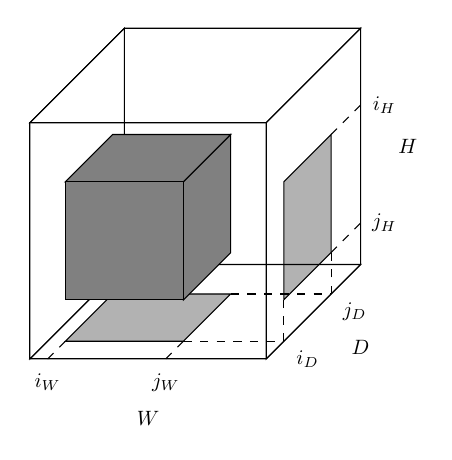
\begin{tikzpicture}[scale=.3, every node/.style={scale=0.75}]
	% \drawline#x1#y1#x2#y2#format
	\def\drawline#1#2#3#4#5{
		\draw[#5] (#1, #2) -- (#3, #4);
	}
	
	% \drawfacef#x#y#size#color#opacity#thickness
	\def\drawfacef#1#2#3#4#5#6{
		\filldraw[fill=#4, fill opacity=#5, #6] 
			(#1, #2) -- ++ (#3, 0) -- ++ (0,  #3) -- ++ (-#3, 0) -- cycle;
	}
	
	% \drawfaceh#x#y#size#color#opacity#thickness
	\def\drawfaceh#1#2#3#4#5#6{
		\filldraw[fill=#4, fill opacity=#5, #6] 
			(#1, #2) -- ++ (#3, 0) -- ++ (#3 * .4,  #3 * .4) -- ++ (-#3, 0) -- cycle;
	}
	
	% \drawfacev#x#y#size#color#opacity#thickness
	\def\drawfacev#1#2#3#4#5#6{
		\filldraw[fill=#4, fill opacity=#5, #6] 
			(#1, #2) -- ++ (#3 * .4,  #3 * .4) -- ++ (0, #3)  -- ++ (-#3 * .4, -#3 * .4) -- cycle;
	}
	
	% \drawcubid#x#y#size#color#opacity#thickness#showall
	\def\drawcubid#1#2#3#4#5#6#7{
		\ifx\\#7\\
			\drawfacev{#1}{#2}{#3}{#4}{#5}{#6} 						% L
			\drawfaceh{#1}{#2}{#3}{#4}{#5}{#6}  					% B
			\drawfacef{#1 + #3 * .4}{#2 + #3 * .4}{#3}{#4}{#5}{#6}	% R
		\fi
		\drawfacev{#1 + #3}{#2}{#3}{#4}{#5}{#6}  					% R
		\drawfaceh{#1}{#2 + #3}{#3}{#4}{#5}{#6}  					% T
		\drawfacef{#1}{#2}{#3}{#4}{#5}{#6} 							% F
	}
	
	
	% big cubid
	\drawcubid{0}{0}{10}{black}{0}{}{}
	
	% line, face and node
	\drawline{0.75}{0}{1.5}{0.75}{dashed}
	\drawline{5.75}{0}{6.5}{0.75}{dashed}
	\drawline{6.5}{0.75}{10.75}{0.75}{dashed}
	\drawline{8.5}{2.75}{12.75}{2.75}{dashed}
	\drawfaceh{1.5}{0.75}{5}{black}{0.3}{}
	
	\drawline{10.75}{0.75}{10.75}{2.5}{dashed}
	\drawline{12.75}{2.75}{12.75}{4.5}{dashed}
	\drawline{12.75}{4.5}{14}{5.75}{dashed}
	\drawline{12.75}{9.5}{14}{10.75}{dashed}
	\drawfacev{10.75}{2.5}{5}{black}{0.3}{}
	
	\node at (0.75, -1) {$i_W$};
	\node at (5.75, -1) {$j_W$};
	\node at (5, -2.5) {$W$};
	
	\node at (11.75, 0) {$i_D$};
	\node at (13.75, 2) {$j_D$};
	\node at (14, 0.5) {$D$};
	
	\node at (15, 10.75) {$i_H$};
	\node at (15, 5.75) {$j_H$};
	\node at (16, 9) {$H$};
	
	% small cuid
	\drawcubid{1.5}{2.5}{5}{gray}{1}{}{n}
\end{tikzpicture}
		\caption{Làm giàu dữ liệu bằng phép trích xuất khối ngẫu nhiên.}
		\label{fig:random_cropping}
	\end{figure}
	Trong luận văn này, chúng tôi làm giàu dữ liệu bằng cách thực hiện cắt ngẫu nhiên một khối dữ liệu từ khối dữ liệu ban đầu như \autoref{fig:random_cropping}. Kích thước của khối dữ liệu đầu ra là ngẫu nhiên. Tuy nhiên, với mong muốn giữ lại được nhiều thông tin khi đưa vào huấn luyện, chúng tôi đặt ràng buộc kích thước cắt cho khối dữ liệu. Gọi $S_H, S_W, S_D$ lần lượt là kích thước chiều cao, chiều rộng và chiều sâu của khối dữ liệu ban đầu; $i_k, j_k$ lần lượt là chỉ số bắt đầu và kết thúc của khối dữ liệu đầu ra trên khối dữ liệu đầu vào theo chiều $k$, với $k\in\{H,W,D\}$. Chúng tôi giới hạn $i_k$ trong khoảng $[0, \lfloor0.1S_k\rfloor)$ và $j_k$ trong khoảng $[\lfloor0.9S_k\rfloor, S_k)$. Sau đó, chúng tôi thực hiện chia không chồng lấp khối dữ liệu có được thành các khối có kích thước $112\times112\times112$ và lần lượt đưa vào huấn luyện.

\section{Xây dựng mã nguồn hệ thống} 
\label{sec:xay_dung_ma_nguon_he_thong}
	\begin{figure}[h!]
		\centering
		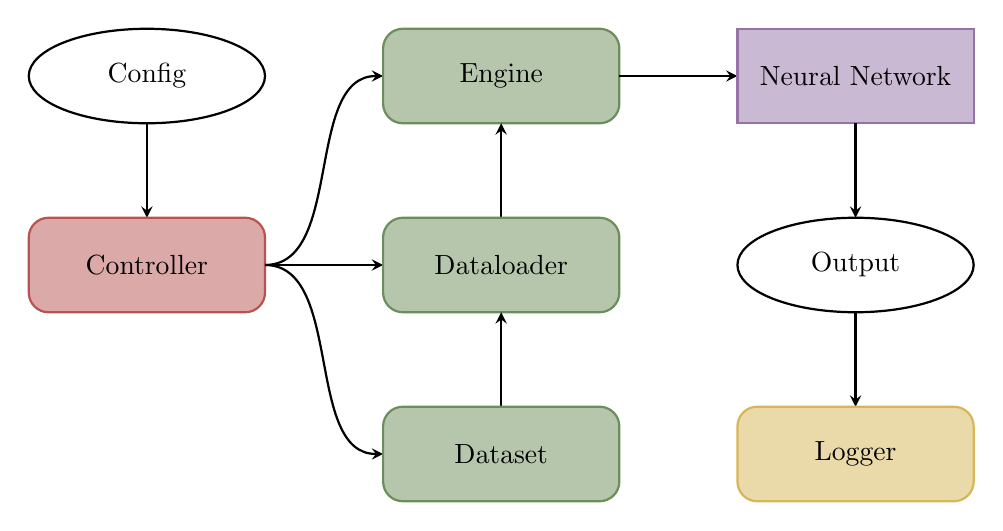
\begin{tikzpicture}[thick, yscale=.8]
	\definecolor{pink}{RGB}{184, 84, 80}
	\definecolor{blue}{RGB}{108, 142, 91}
	\definecolor{purple}{RGB}{150, 115, 166}
	\definecolor{yellow}{RGB}{214, 182, 86}
	
	% \drawroundedrectangle#x#y#width#height#corner#color$label
	\def\drawroundedrectangle#1#2#3#4#5#6#7{
		\fill[#6, fill opacity=.5, draw=#6, rounded corners=#5cm] (#1, #2) -- ++ (#3, 0) -- ++ (0, #4) -- ++(-#3, 0) -- cycle;
		\node at (#1 + #3 / 2, #2 + #4 / 2) {#7};
	}
	
	% \drawellipse#xcenter#ycenter#radiuswidth#radiusheight#label
	\def\drawellipse#1#2#3#4#5{
		\draw  (#1, #2) ellipse (#3 and #4) node {#5};
	}
	
	% diagram
	\drawellipse{1.5}{8.75}{1.5}{0.75}{Config}
	\draw[-stealth] (1.5, 8) -- (1.5, 6.5);
	\drawroundedrectangle{0}{5}{3}{1.5}{.25}{pink}{Controller}
	\draw[-stealth] (3, 5.75) .. controls (4, 5.75) and (3.5, 8.75) .. (4.5, 8.75);
	\draw[-stealth] (3, 5.75) -- (4.5, 5.75);
	\draw[-stealth] (3, 5.75) .. controls (4, 5.75) and (3.5, 2.75) .. (4.5, 2.75);
	\drawroundedrectangle{4.5}{8}{3}{1.5}{.25}{blue}{Engine}
	\draw[-stealth] (6, 6.5) -- (6, 8);
	\drawroundedrectangle{4.5}{5}{3}{1.5}{.25}{blue}{Dataloader}
	\draw[-stealth] (6, 3.5) -- (6, 5);
	\drawroundedrectangle{4.5}{2}{3}{1.5}{.25}{blue}{Dataset}
	\draw[-stealth] (7.5, 8.75) -- (9, 8.75);
	\drawroundedrectangle{9}{8}{3}{1.5}{0}{purple}{Neural Network}
	\draw[-stealth] (10.5, 8) -- (10.5, 6.5);
	\drawellipse{10.5}{5.75}{1.5}{0.75}{Output}
	\draw[-stealth] (10.5, 5) -- (10.5, 3.5);
	\drawroundedrectangle{9}{2}{3}{1.5}{0.25}{yellow}{Logger}
\end{tikzpicture}
		\caption[Kiến trúc của bộ mã nguồn \textit{Insight Deep Learning}]{Kiến trúc của bộ mã nguồn \textit{Insight Deep Learning} \sourcefig{\cite{nhatson2019tumor}}.}
		\label{fig:insignt_deep_leaning}
	\end{figure}
	Để thuận tiện hơn trong quá trình thí nghiệm cũng như giúp hệ thống có thể dễ dàng phát triển và bảo trì trong tương lai, chúng tôi sử dụng bộ mã nguồn \textit{Insight Deep Learning} của GVLab được hiện thực bằng PyTorch\index{PyTorch} với những ưu điểm sau đây:
	\begin{itemize}
		\setlength\itemsep{0em}
		\item Bộ mã được tổ chức thành các khối chức năng rõ ràng, hợp lý giúp dễ dàng trong quá trình sử dụng, mở rộng và bảo trì.
		\item Hỗ trợ huấn luyện song song trên nhiều GPU.
		\item Hỗ trợ giám sát thời gian thực trong quá trình huấn luyện với nhiều dạng khác nhau như biểu đồ, chữ,\ldots
		\item Trong trường hợp quá trình huấn luyện bị dừng đột ngột vì lý do không mong muốn, hệ thống cho phép phục hồi quá trình huấn luyện nhờ khả năng sao lưu và khôi phục trạng thái trong quá trình huấn luyện.
		\item Các siêu tham số và các cài đặt cho quá trình huấn luyện được quản lí trong một tệp YAML\footnote{YAML là một chuẩn tuần tự hóa dữ liệu cho nhiều ngôn ngữ lập trình dưới dạng chữ, giúp con người dễ dàng đọc, hiểu.}\nomenclature{YAML}{YAML Ain't Markup Language}. Nhờ vậy, khi cần thay đổi thông số cài đặt, lập trình viên chỉ cần chỉnh sửa thông tin trong tệp này.
		\item Sử dụng chung một bộ mã nguồn với cùng một ngôn ngữ, cấu trúc cho phép các thành viên của GVLab hợp tác với nhau thuận lợi hơn cũng như quá trình kế thừa và phát triển mã nguồn dễ dàng hơn.
	\end{itemize}
	Kiến trúc của bộ mã được mô tả trong \autoref{fig:insignt_deep_leaning}. Controller là khối được thực thi đầu tiên với các thông số lấy từ khối Config. Controller có nhiệm vụ điều khiển các thành phần Dataset, DataLoader, Engine làm việc với nhau. Dataset xử lí tất cả các tác vụ liên quan đến dữ liệu như đọc tệp, làm giàu dữ liệu. DataLoader quản lí số lượng mẫu và cách mà mỗi mẫu được đưa vào huấn luyện. Engine sẽ lấy dữ liệu từ DataLoader để đưa vào Neural Network. Phụ thuộc vào loại Engine, đầu ra của Neural Network sẽ được dùng để tính giá trị lỗi, đưa ra kết quả dự đoán hoặc để tính toán các độ đo ghi vào Logger.
	
	\newpage
	Trong luận văn này, chúng tôi kế thừa và phát triển bộ mã để phục vụ cho quá trình xây dựng hệ thống. Những bổ sung chính mà chúng tôi thực hiện trên bộ mã liên quan đến các mô hình trong các công trình liên quan chúng tôi tham khảo và khả năng làm việc với dữ liệu 3D.
	
\section{Đặc tả phần cứng}
\label{sec:dac_ta_phan_cung}
	Huấn luyện mạng học sâu với một lượng lớn dữ liệu đòi hỏi sức mạnh tính toán cao để công tác huấn luyện diễn ra nhanh chóng và hiệu quả. Để đáp ứng yêu cầu đó, trong luận văn này, chúng tôi sử dụng hệ thống máy tính hiệu năng cao (HPCC\nomenclature{HPCC}{High Performance Computing Center}) được hỗ trợ bởi GVLab \nomenclature{GVLab}{Graphics and Computer Vision Laboratory} nhằm mục đích huấn luyện hệ thống. \autoref{tab:dac_ta_phan_cung} mô tả chi tiết thông số cấu hình hệ thống mà chúng tôi đã sử dụng.
	\begin{table}[h!]
		\centering
		\caption{Thông tin phần cứng hệ thống máy tính.}
		\label{tab:dac_ta_phan_cung}
		\begin{tabular}{@{\hspace{7mm}}c@{\hspace{7mm}}l@{\hspace{8mm}}l@{\hspace{5mm}}}
			\toprule
			\textbf{STT} & \textbf{Phần cứng} & \textbf{Cấu hình}\\ \midrule
			1	& CPU       & Intel(R) Xeon(R) CPU E5-2640 v3 @ 2.60GHz 16 cores \\[1mm]
			2	& RAM\nomenclature{RAM}{Random Access Memory}       & 128 GB                                    \\[1mm]
			3	& GPU       & NVIDIA Tesla P100 16GB                    \\ \bottomrule
		\end{tabular}
	\end{table}
	\vspace{-3mm}

\section{Hậu xử lý kết quả phân đoạn} 
\label{sec:hau_xu_ly_ket_qua_phan_doan}
	Hệ thống mạch máu là một cấu trúc khép kín. Nếu coi hệ thống này là một đối tượng trong không gian thì nó sẽ gói gọn trong một thành phần liên thông duy nhất. Đối với hệ thống mạch máu trong khối ảnh CT của một phần cơ thể, cụ thể với giả thiết được nêu ra trong \autoref{subsec:trich_xuat_thanh_phan_gan}, hệ thống này sẽ bao gồm một số lượng hữu hạn\footnote{Có khoảng 6 nhánh mạch máu trong cơ quan gan với 3 nhánh xuất phát từ tĩnh mạch chủ và 3 nhánh còn lại xuất bạn từ tĩnh mạch cửa.}các nhánh mạch máu mà mỗi nhánh này là một thành phần liên thông.
	
	Hệ thống mạch máu có được từ kết quả phân đoạn không thể tránh khỏi có những điểm ảnh bị phân đoạn sai. Đặc biệt, những điểm ảnh rời rạc không thuộc mạch máu bị phân đoạn sai sẽ làm xấu đi kết quả thí nghiệm. Nhằm cải thiện kết quả phân đoạn, chúng tôi đề xuất thực hiện xác định các thành phần liên thông trong cây mạch máu được sinh ra. Sau đó, lần lượt loại bỏ những thành phần liên thông có tổng số lượng điểm ảnh là nhỏ nhất sao cho tổng số lượng điểm ảnh bị loại bỏ không vượt quá 10\% tổng số điểm ảnh được phân đoạn là mạch máu. 
	
	Việc xác định các thành phần liên thông và loại bỏ các thành phần liên thông nhỏ được chúng tôi thực hiện thông qua các hàm đã được hiện thực sẵn trong ngôn ngữ Python lần lượt là hàm \verb/label/ trong gói \verb/ndimage.measurements/ của thư viện \verb/scipy/ và hàm \verb/histogram/ và \verb/argsort/ của thư viện \verb/numpy/.
	
\newpage
\section{Trực quan hoá kết quả thí nghiệm} 
\label{sec:truc_quan_hoa_ket_qua_thi_nghiem}
	Sau khi có kết quả phân đoạn mạch máu cũng như đường chính giữa và điểm phân nhánh mạch máu. Chúng tôi thực hiện trực quan hoá kết quả thông qua hai bước.
	
	Bước thứ nhất, chúng tôi tiến hành trích xuất lưới bề mặt đối tượng cần trực quan bằng thư viện VTK\index{VTK}. Bước này nhằm giảm thiểu khối lượng tính toán trên GPU lúc hiển thị, bởi nếu sử dụng ngay kết quả đầu ra của hệ thống là mảng ba chiều thì khối lượng tính toán cần thực hiện trên GPU là rất lớn. Từ đó, cải thiện chất lượng hiển thị nhờ tăng số lượng khung hình trên giây và việc trực quan sẽ mượt mà hơn.
	
	Bước thứ hai, hiển thị lưới bề mặt của đối tượng trên ứng dụng Slicer\index{Slicer}. Với ứng dụng Slicer, chúng tôi có thể hiển thị chồng kết quả phân đoạn và nhãn phân đoạn tương ứng lên nhau, từ đó có thể dễ dàng so sánh sự sai khác của kết quả phân đoạn. \autoref{fig:slicer_visualize} là ví dụ về việc sử dụng ứng dụng Slicer để trực quan hệ thống tĩnh mạch của một bệnh nhân.
	\vspace{2mm}
	\begin{figure}[h!]
		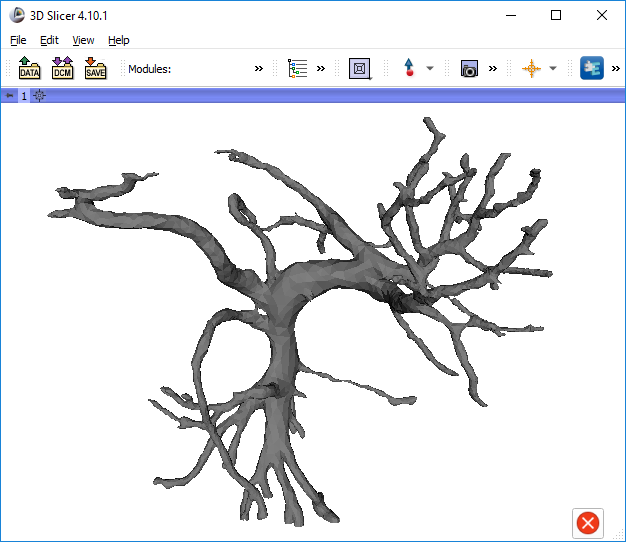
\includegraphics[width=\textwidth]{figures/slicer_visualize}
		\caption{Trực quan hoá kết quả trên ứng dụng Slicer.}
		\label{fig:slicer_visualize}
	\end{figure}